\section{Introduction}
\label{sec:intro}
Neural network models have led to improved performance 
in natural language processing tasks, and helped achieve
the state-of-the-art results in a large variety of tasks
such as natural language inference~\cite{bowmanlarge,bowman2015large,wang2018glue}, 
argumentation~\cite{niven2019probing}, commonsense
reasoning~\cite{mostafazadeh2016corpus,roemmele2011choice,zellers2018swag}, 
reading comprehension~\cite{lai2017race}, question answering~\cite{talmor2019commonsenseqa} 
and dialogue analysis~\cite{lowe2015ubuntu}. 
However, recent work~\cite{gururangan2018annotation,sanchez2018behavior,poliak2018hypothesis}
 has identified statistical spurious patterns like sentiment, word overlap
and even shallow ngram tokens in benchmark datasets 
are predictive of the correct answer. 
%\KZ{Don't use absolute mm width in figures. Use relative length instead!}
\begin{figure}[th]
\centering
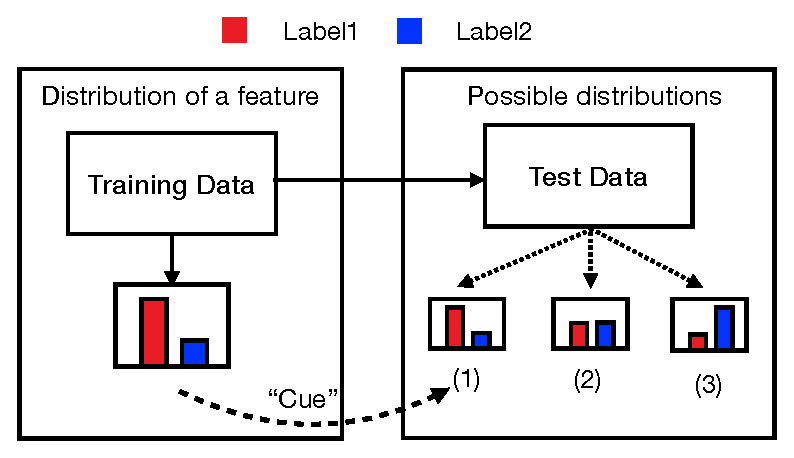
\includegraphics[width=0.6\columnwidth]{picture/cue_def.eps}
\caption{Example of a cue.}
\label{fig:cue_def}
\end{figure}
We call these patterns or features as \textbf{cues} which can be 
defined as if a pattern is unbalanced with different 
labels in both training and test dataset, 
and the distributions are similar, then we will call that a cue.
We illustrate this in~\figref{fig:cue_def}. 
Once these cues are neutralized in 
stress test~\cite{naik2018stress,mccoy2019right}, 
models perform poorly, suggesting 
that evaluating on those datasets may overestimate the true capability of 
models or even constrain the learning  of models. 



Existing techniques to improve the quality of the datasets 
include data filtering, data augmentation and stress test generation. 
First, the data filtering model~\cite{bras2020adversarial} 
produces a reduced dataset with fewer spurious patterns through iteratively 
training on complex neural network models. However, it strongly 
depends on the specific models to make filter decision which 
adapts the dataset toward a few models but cannot generalize to future
models. 
Second, collecting more data manually for data augmentation
is too expensive, thus some work~\cite{wang2019if,mccoy2019right} automatically generate 
more training data in which neutralizes some 
spurious cues with designed logic rules. 
But these methods only focus on the word overlap problem 
which is especially serious in certain dataset, e.g., MNLI~\cite{wang2018glue}. 
They can't be generalized to other datasets with different kinds of
cues. Third, the methods~\cite{naik2018stress,mccoy2019right} 
that generate stress test aimed at breaking the spurious cues information leakage 
between training and testing dataset. 
%\KZ{You mentioned cues a few sentences ago, and now you are
%defining cues? This def is not good enough i think: 
%We give this kind of cue a definition that if 
%a token is unbalanced with different labels in both training and test dataset, 
%and the distributions are similar, we will call that is a cue.
%We illustrate this in~\figref{fig:cue_def}. 
But the stress data generation must find 
specific cues first and design the new dataset manually, 
like stress test for cue ``not"~\cite{schuster2019towards}
in ARCT dataset~\cite{niven2019probing}.
% which is expensive.
Few studies have focused on the description of the extent 
to which datasets contain spurious cues, and improve these datasets 
in a way that can benefit the evaluation of all kinds of models. 

%\KZ{I think you talk too much details in the following 4 paras.
%Cut them down to half of the size! Talk only generally, enough for ppl
%to understand at a high level!
%This para you define the kind of datasets you are targeting.}
In this paper,
We propose a computationally efficient framework
which can be used to evaluate
% all kinds of 
%\KZ{What you do mean by that: multiple choice 
%datasets}
a broader range of multiple choice datasets. 
%Moreover, a by-product of the framework is to produce higher quality training
%data that can be used to improve the strength of the models to some extent.
%The multiple choice datasets that we are targeting in this paper should involve a ``premise'', 
%a ``hypothesis'' and a ``label'' in each instance. 
An multiple choice example is shown below:
\begin{example}\label{exp:snli}
An example in SNLI.

\noindent
\textbf{Premise}: A swimmer playing in the surf watches a low flying airplane headed inland. 

\noindent
\textbf{Hypothesis}: Someone is swimming in the sea.

%\textbf{alternatives}: Entailment Contradiction  Neutral 

\noindent
\textbf{Label}: a) Entail. b) Contradict.  c) Neutral.
\end{example}
%\KZ{Shall we call it a label?} 
We should choose the correct label from the alternatives ``entailment'', 
``contradiction'' and ``neutral'' for the 
task of determining whether a \textbf{premise} sentence 
entails (i.e., implies the truth of) a \textbf{hypothesis} sentence.
% ``premise'' and ``hypothesis'' can 
%have different relations on labels.
%\KZ{The hypothesis is the choice right?
%I don't think u have explain the MCQ properly..}
Though not all multiple choice datasets 
%that we are targeting in this paper should
 involve a premise, 
a hypothesis and a label in each instance,
%Any multiple choice instance
they can be unified to this form. We will describe the 
normalization in~\secref{sec:approach}.
%We explore 12 datasets on 6 tasks 
% in ~\figref{fig:datasets_exp} 
%which
%are in this general form. This formulation will be introduced in~\secref{sec:approach}.
%They can be classified into three types of tasks. 
%The first type are the NLI tasks which keep the original format. 
%The second type, including ARCT~\cite{niven2019probing}., ARCT\_adv\cite{schuster2019towards}, 
%RACE~\cite{lai2017race}, and Reclor~\cite{yu2020reclor}, 
%\KZ{Don't understand: only has the premise and the hypothesis without the choices.}
%For example, in~\figref{fig:datasets_exp}, 
%ARCT dataset have \textbf{Reason} and \textbf{Claim} which requires to select the right warrant between them. 
%RACE and Reclor includes text and questions which will be seen as ``premise''. 
%The label for each choice is 
%``right'' or ``wrong'' for whether this choice is the correct one.
%The third type contains Ubuntu~\cite{lowe2015ubuntu}, COPA~\cite{roemmele2011choice}, ROCStory~\cite{mostafazadeh2016corpus}, SWAG~\cite{zellers2018swag} and 
%CQA~\cite{talmor2019commonsenseqa}, similar with the former type 
%\KZ{but with only one part (either premise or hypothesis) before choices.}
 %the former four sentences of a story in ROCStory 
 %dataset~\cite{mostafazadeh2016corpus} can be identified as ``premise'' ,  
 %each alternative is identified as ``hypothesis''.   if the alternative is the correct ending of the story, 
 %the corresponding ``label'' is \textbf{right} versus \textbf{wrong}. 

%\KZ{This para you define cues very abstractly, and using simple linear
%models you can separate any given dataset into easy and hard part
%and thus evaluate the ``biasness'' and ``quality'' of the dataset.}
Given the instances containing premise, hypothesis and label, 
we calculate the correlation score between cues first. 
In this paper, we focus on shallow cues such as the distribution of
unigrams which may help the model obtain the correct answer 
without truly understanding the 
context~\cite{naik2018stress,schuster2019towards}. 
%Detailed description about different cues is in ~\secref{sec:related}. 
%For investigating the unbalance scores between cues and the labels,
%we leverage several correlation methods such as point-wise mutual information(PMI).
%\KZ{This para is about evaluating the neural models using the easy and hard
%split of the test set.}
%Second, by using simple linear models with the bias score of cues we can separate 
Second, to  evaluate 
the ``biasness'' and ``quality'' of the dataset, 
we device a very simple model using only the cues to try to
solve the questions in the dataset. 
We separate the dataset into easy and hard parts based on 
whether the question can be correctly answered
using the cue features only. The proportion of hard part over the whole
data indicates the quality of the dataset (the most the hard part is the better the
dataset).
%Thus we can
%separate the original dataset into easy and hard part with 
%the bias score feature of cues
%any given dataset into easy and hard part
%and thus we can evaluate the ``biasness'' and ``quality'' of the dataset. 
Meanwhile, 
%the samples of original dataset are automatically 
%separated into easy and hard part  on the basis of whether can be correct chosen 
%with the bias features only.
%generated 
this hard-easy split can be used to
estimate the real performance of a model. 
A large difference in the performance on these two parts indicates
the weakness of the model.
%using simple and cost-effective linear classification models 
%on the simple cue features,
%which trained with unbalanced score of cues to several benchmark datasets across 
%various tasks and domains. 
%We evaluate the effectiveness of our methods with the 
%deviation between our results and random selection results. 
%Simultaneously, the test set can be divided into two parts: \textbf{easy} and \textbf{hard}. 
 %\textbf{balance} and \textbf{imbalance} are relative rather than absolute. 
%\KZ{Improving the neural models by splitting the training set.} 
Finally, we experimented with splitting the training data 
in to easy and hard parts, too
and show that by filtering out the easy questions from training data,
there is a potential to improve the robustness of the model by ``forcing'' it
to steer its focus away from trivial cues. 

%The training data can be separated into $n$ parts, test on one part and training 
%the model on the rest for each time. 
%The filtered part contains the instances 
%which can not be correctly chosen.
%The filtered data will be used to train a better model for target tasks. 

In summary, this paper makes the following contributions:
%\KZ{These contribs need to be revised right?}
\begin{itemize}
\item We provide a light-weight and effective method to 
evaluate the unigram related cues of multiple choice datasets (\secref{sec:experiment1}) .
%(\secref{sec:result}).

\item We separate the test dataset two parts according to  
the extent of unbalance. 
We can measure the model's robustness and real performance 
by differences of the results on the easy and hard part of the test data~(\secref{sec:experiment2}).
\item We further split the training set using a heuristics that allows to
train the model to better accuracy on the hard test data (\secref{sec:experiment3}). 

\end{itemize}
% (\secref{sec:result}).

%\item We filter the training data and get a better performance on the \textbf{hard} dataset.
%to get a high quality training dataset which
 %is possibly closer to the intended task. 

















